% Created 2022-09-05 Mon 18:27
% Intended LaTeX compiler: xelatex
\documentclass[8pt]{article}
  \usepackage[letterpaper, portrait, margin=1in]{geometry}
  \usepackage[utf8]{inputenc}
  \usepackage[T1]{fontenc}
  \usepackage{amsmath}
  \usepackage{amssymb}
  \usepackage{hyperref}
  \hypersetup{colorlinks=true}
  \usepackage{tcolorbox}
% http://tug.ctan.org/macros/latex/contrib/minted/minted.pdf
  \usepackage[cache=false]{minted}
  \setminted{breaklines=true, breakanywhere=true}
% \usemintedstyle{paraiso-light} % pygmentize -L styles
% \usemintedstyle{emacs} % pygmentize -L styles
% \usemintedstyle{colorful} % pygmentize -L styles
% \usemintedstyle{rainbow_dash} % pygmentize -L styles
  \usemintedstyle{tango} % pygmentize -L styles
% https://tex.stackexchange.com/questions/112559/box-around-minted-environment
% https://ctan.math.utah.edu/ctan/tex-archive/macros/latex/contrib/tcolorbox/tcolorbox.pdf
  \BeforeBeginEnvironment{minted}{\begin{tcolorbox}[colframe=black!85!white, colback=black!5!white, boxrule=0.3mm]}
  \AfterEndEnvironment{minted}{\end{tcolorbox}}
  \usepackage{enumitem}
  \setitemize{itemsep=0.5pt}
  \usepackage{fancyhdr}
  \pagestyle{fancy}
  \fancyhf{}
  \usepackage{titling} % allows 	hetitle 	heauthor 	hedate
  \usepackage{lastpage}
  \rhead{\theauthor}
  \lhead{\thetitle}
% Disable pageref being a link https://tex.stackexchange.com/a/4599
  \rfoot{\thepage{} of \pageref*{LastPage}}
  \linespread{1}
  \setlength{\parindent}{0pt}
  \setlength{\parskip}{0.5em plus 0.1em minus 0.2em}
  \hypersetup{pdfborder=0 0 0}
  \setcounter{secnumdepth}{0}
%  \usepackage{fontspec}
%  \setmainfont[]{IBM Plex Sans}
%  \setmonofont[]{Iosevka SS14}

\usepackage{graphicx}
\usepackage{longtable}
\usepackage{wrapfig}
\usepackage{rotating}
\usepackage[normalem]{ulem}
\usepackage{amsmath}
\usepackage{amssymb}
\usepackage{capt-of}
\usepackage{hyperref}
\usepackage{fontspec}
\setmainfont[]{IBM Plex Sans}
\setmonofont[]{Iosevka SS14}
\author{Jonathan Fung}
\date{07/12/22}
\title{Flights}
\hypersetup{
 pdfauthor={Jonathan Fung},
 pdftitle={Flights},
 pdfkeywords={},
 pdfsubject={},
 pdfcreator={Emacs 29.0.50 (Org mode 9.5.4)},
 pdflang={English}}
\begin{document}

\maketitle
\tableofcontents

\begin{latex}
\pagebreak
\end{latex}
\section{Import}
\label{sec:org7402cf0}
Source: \href{https://github.com/rfordatascience/tidytuesday/tree/master/data/2022/2022-07-12}{tidytuesday - July 12, 2022}

\begin{minted}[]{r}
library(tidyverse)
library(fpp3)
tuesdata <- tidytuesdayR::tt_load('2022-07-12')
flights <- tuesdata$flights

names(flights)
\end{minted}

\begin{center}
\begin{tabular}{l}
YEAR\\
MONTH\_NUM\\
MONTH\_MON\\
FLT\_DATE\\
APT\_ICAO\\
APT\_NAME\\
STATE\_NAME\\
FLT\_DEP\_1\\
FLT\_ARR\_1\\
FLT\_TOT\_1\\
FLT\_DEP\_IFR\_2\\
FLT\_ARR\_IFR\_2\\
FLT\_TOT\_IFR\_2\\
Pivot Label\\
\end{tabular}
\end{center}

This dataset is a daily time series on each airport, with each record having total IFR movement, departures, and arrivals, from both "Network Manager" (1) and "Airport Operator" (2).

\begin{minted}[]{r}
head(flights[,1:8])
\end{minted}

\begin{center}
\begin{tabular}{rrlrlllr}
2016 & 1 & JAN & 2016-01-01 & EBAW & Antwerp & Belgium & 4\\
2016 & 1 & JAN & 2016-01-01 & EBBR & Brussels & Belgium & 174\\
2016 & 1 & JAN & 2016-01-01 & EBCI & Charleroi & Belgium & 45\\
2016 & 1 & JAN & 2016-01-01 & EBLG & Liège & Belgium & 6\\
2016 & 1 & JAN & 2016-01-01 & EBOS & Ostend-Bruges & Belgium & 7\\
2016 & 1 & JAN & 2016-01-01 & EDDB & Berlin - Brandenburg & Germany & 98\\
\end{tabular}
\end{center}
\begin{latex}
\pagebreak
\end{latex}
\section{Utils}
\label{sec:orgdd2aa01}
Define \texttt{assignRegion}, using the \href{https://en.wikipedia.org/wiki/Regions\_of\_Europe}{CIA - The World Factbook} to assign European regions to states. Also define \texttt{cleanState}, which cleans up some state names to work with the \texttt{rlnaturalearth} package.

\begin{minted}[]{r}
assignRegion <- function (s) {
  region <- case_when(
s == "Belgium" ~ "Western Europe",
#...
s == "Israel" ~ "Not Europe" # Middle East
	      )
  return(region)
}


# Convert STATE_NAMEs format in flights to work with rnaturalearth
cleanState <- function (s) {
  state <- case_when(
s == "Bosnia and Herzegovina" ~ "Bosnia and Herz.",
#...
s == "Türkiye" ~ "Turkey",
TRUE ~ s
	      )
  return(state)
}
\end{minted}

\begin{minted}[]{r}
assignRegion("Netherlands")
cleanState("Czech Republic")
\end{minted}

\begin{verbatim}
[1] "Western Europe"
[1] "Czech Rep."
\end{verbatim}


\begin{latex}
\pagebreak
\end{latex}
\section{Explore}
\label{sec:org51c57d1}

The huge dip in the beginning of 2020 is when the COVID-19 Pandemic lockdowns started to hit the world. Before that, we see a pretty consistent seasonality. After, there is still seasonality, but with significant growth trends. The order across regions also persists during the pandemic.

\begin{minted}[]{r}
by_region <- flights %>%
  mutate(region = assignRegion(STATE_NAME)) %>%
  group_by(FLT_DATE, region) %>%
  summarise(tot = sum(FLT_TOT_1), .groups = "keep") %>%
  mutate(FLT_DATE = as.Date(FLT_DATE)) %>%
  as_tsibble(key = region, index = FLT_DATE)

## https://dcl-data-vis.stanford.edu/time-series.html#one-response-variable
by_region %>% autoplot(tot) +
  geom_text(aes(label = region),
	    data = by_region %>% filter(FLT_DATE == "2022-05-31"),
	    color = "black",
	    hjust = 0,
	    size = 3,
	    nudge_x = 5,
	    angle = 40) +
  xlab("Day") + ylab("Sum of daily total IFR movements") +
  ggtitle("Plot by Region") +
  scale_x_date(limits = as.Date(c("2016-01-01", "2023-02-01"))) +
  theme(legend.text=element_text(size=6),
	legend.position="none")
\end{minted}

\begin{center}
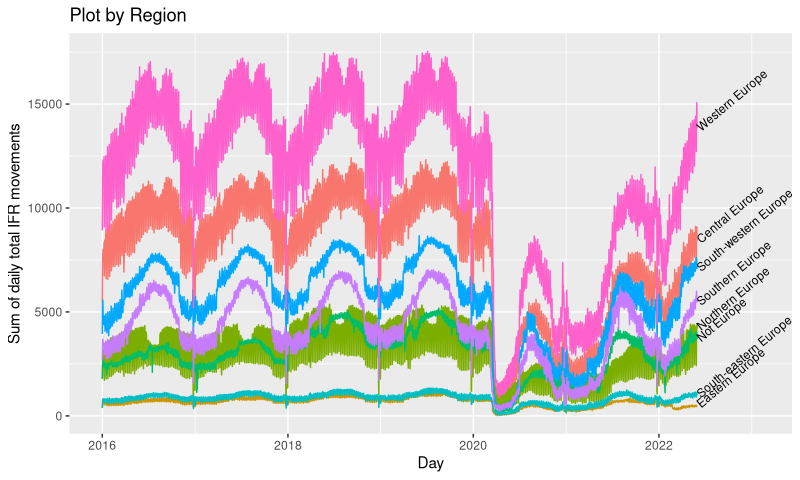
\includegraphics[width=.9\linewidth]{./media/tot_region.png}
\end{center}

\begin{latex}
\pagebreak
\end{latex}

For clarity, we can view the same data, but summed over regions.

\begin{minted}[]{r}
TOT_sum <- flights %>%
  group_by(FLT_DATE) %>%
  summarise(tot = sum(FLT_TOT_1)) %>%
  mutate(FLT_DATE = as.Date(FLT_DATE)) %>%
  as_tsibble(index = FLT_DATE)

TOT_sum %>% autoplot(tot) +
  xlab("Day") + ylab("Sum of daily total IFR movements") +
  ggtitle("Sum of total IFR movements")
\end{minted}

\begin{center}
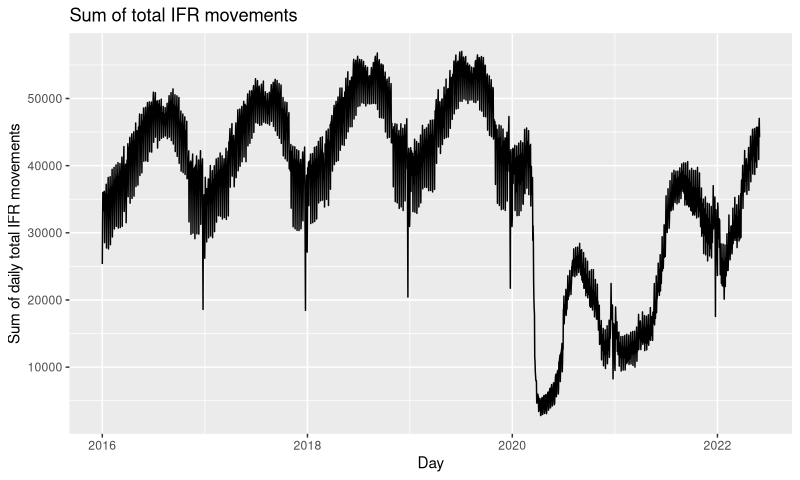
\includegraphics[width=.9\linewidth]{./media/tot_sum.png}
\end{center}

\begin{latex}
\pagebreak
\end{latex}

STL Decomposition clearly shows that this data exhibits trend, year-seasonality, and week-seasonality. Non-patterns are caught in the \emph{remainder}, especially the large dip during the start of COVID-19.

\begin{minted}[]{r}
TOT_sum %>%
  model(stl = STL(tot)) %>%
  components() %>% autoplot() + xlab("Day") +
  ggtitle("STL Decomposition")
\end{minted}

\begin{center}
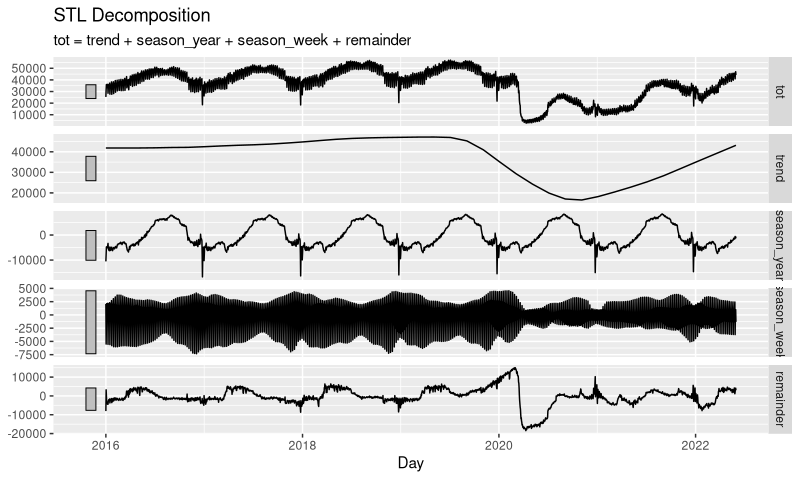
\includegraphics[width=.9\linewidth]{./media/tot_sum_decomp.png}
\end{center}

\begin{latex}
\pagebreak
\end{latex}
\section{Inference}
\label{sec:org1a1f9ac}
STL decomposition also allows us to look at behavior a time series exhibits, particularly seasonality and how strong it trends.

\begin{minted}[]{r}
by_region %>%
  features(tot, feat_stl) %>%
  ggplot(aes(x = trend_strength,
	     y = seasonal_strength_week,
	     col = region)) +
  geom_point(size = 4) +
  ggtitle("Weekly Seasonality  vs Trend Strength by region")
\end{minted}

\begin{center}
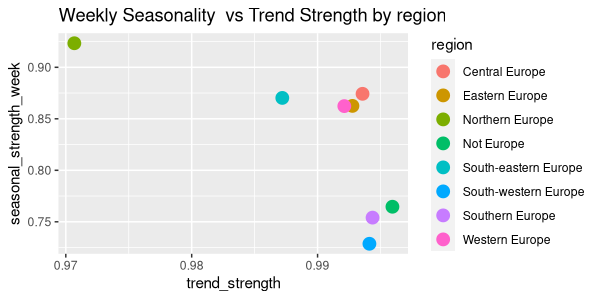
\includegraphics[width=.9\linewidth]{./media/feat_region.png}
\end{center}

\begin{latex}
\pagebreak
\end{latex}

This can also be applied to every state:

\begin{minted}[]{r}
# https://stackoverflow.com/questions/30372368/adding-empty-graphs-to-facet-wrap-in-ggplot2
feats_state <- flights %>%
  group_by(FLT_DATE, STATE_NAME) %>%
  summarise(tot = sum(FLT_TOT_1), .groups = "keep") %>%
  mutate(FLT_DATE = as.Date(FLT_DATE)) %>%
  as_tsibble(key = STATE_NAME, index = FLT_DATE) %>%
  features(tot, feat_stl) %>%
  mutate(georegion = assignRegion(STATE_NAME)) %>%
  mutate(STATE_NAME = cleanState(STATE_NAME))

feats_state %>%
  ggplot(aes(x = trend_strength,
	     y = seasonal_strength_week,
	     label = STATE_NAME)) +
  ggtitle("Features - By State, faceting on Region") +
  geom_point() +
  geom_text(size = 2.5, hjust = 0, nudge_x = 0.001) +
  facet_wrap(.~factor(georegion,
		      # order levels to spatially arange facets
		      levels=c('', 'Northern Europe', 'Not Europe',
			       'Western Europe', 'Central Europe', 'Eastern Europe',
			       'South-western Europe', 'Southern Europe', 'South-eastern Europe')),
	     drop=FALSE)

\end{minted}

\begin{center}
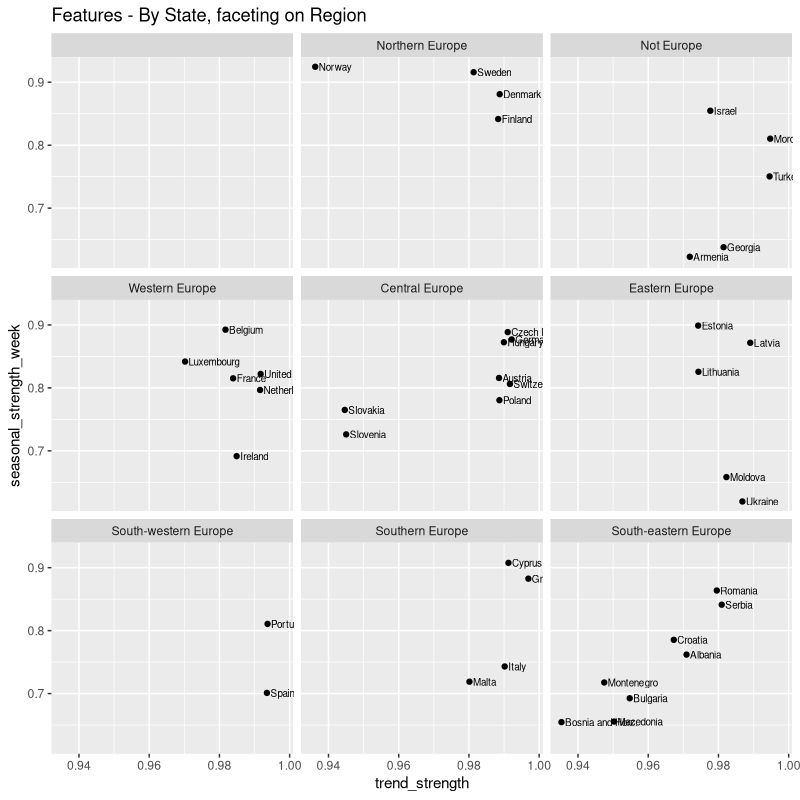
\includegraphics[width=.9\linewidth]{./media/feat_state.png}
\end{center}

All states have a fairly high trend-strength, never less than \texttt{0.94}. On the other hand, Northern, Western, and Central Europe have high weekly seasonality.

\begin{latex}
\pagebreak
\end{latex}
\section{GIS}
\label{sec:org09651cf}
The previous result can be visualized using some GIS libraries.

\begin{minted}[]{r}
library("sf")
library("rnaturalearth")
library("rnaturalearthdata")
\end{minted}

\begin{minted}[]{r}
# "name" is rnaturalearth refers to a country
feats_state_gis <- feats_state %>% rename(name = STATE_NAME)

earth <- ne_countries(scale = "medium", returnclass = "sf")
eu <- right_join(earth, feats_state_gis, by = "name")
eu_coords = data.frame(name = eu$name, st_coordinates(st_centroid(eu)))

ggplot(eu) +
  # relevant: trend_strength, seasonal_strength_week, linearity, curvature
  geom_sf(aes(fill = seasonal_strength_week)) +
  geom_label(data = eu_coords, aes(x=X, y=Y, label = name), size = 2, alpha = 0.5) +
  coord_sf(xlim = c(-17, 45), ylim = c(22, 70)) + # 78 <> 70 to cut off top off Norway (Svalbard)
  ggtitle("Mapped Features") +
  theme(legend.position = c(1,0),
	legend.justification = c(1,0),
	legend.box.margin = margin(5, r = 5, b = 5, unit = "mm"),
	legend.direction = "horizontal",
	plot.title = element_text(vjust = -10, hjust = 0.5, size = 16)
	)
\end{minted}

\begin{center}
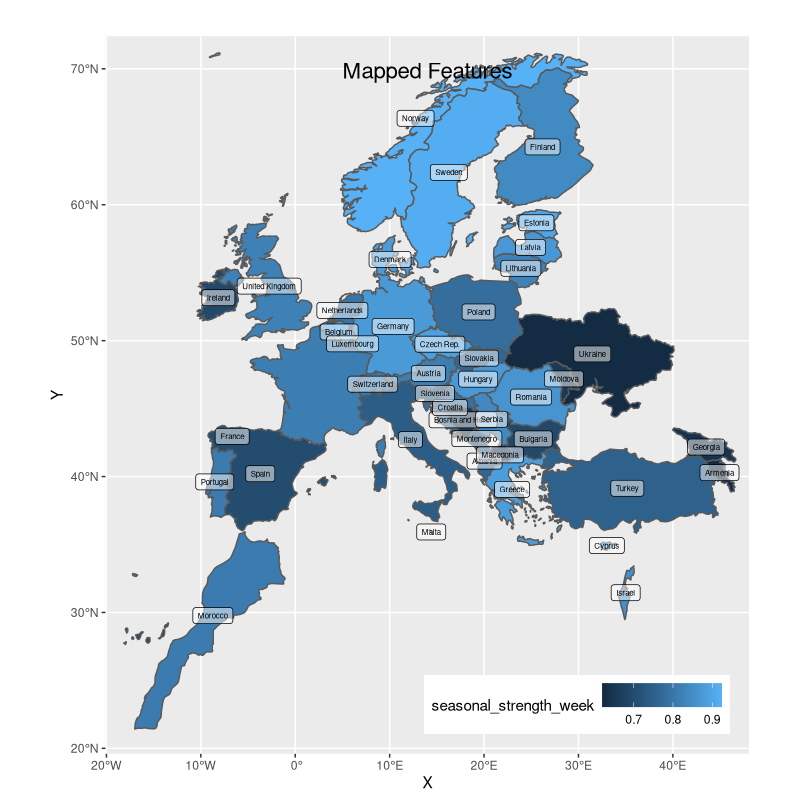
\includegraphics[width=.9\linewidth]{./media/feat_gis.png}
\end{center}

\subsection{References}
\label{sec:org38c36f2}
\begin{itemize}
\item \href{https://r-spatial.org/r/2018/10/25/ggplot2-sf.html}{Drawing beautiful maps programmatically with R, sf and ggplot2 — Part 1: Basics}

\begin{latex}
\pagebreak
\end{latex}
\end{itemize}
\section{Forecasting}
\label{sec:org5b6219c}

For fun, we can build 3 \emph{ARIMA} models, on data before the lockdowns (< March 2020), after/during (> April 2020), and overall. Box-Cox transformations will also be applied to stabilize results. Forecasts are calculated for half a year.

\begin{minted}[]{r}
lambda_bef <- TOT_sum %>%
  filter_index(. ~ "2020-02") %>%
  features(tot, features = guerrero) %>% pull(lambda_guerrero)
lambda_dur <- TOT_sum %>%
  filter_index("2020-04" ~ .) %>%
  features(tot, features = guerrero) %>% pull(lambda_guerrero)
lambda_ovr <- TOT_sum %>%
  features(tot, features = guerrero) %>% pull(lambda_guerrero)

H <- 180

before <- TOT_sum %>% filter_index(. ~ "2020-02") %>%
  model("Before Pandemic" = ARIMA(box_cox(tot, lambda_bef))) %>% forecast(h = H)
during <- TOT_sum %>% filter_index("2020-04" ~ .) %>%
  model("During Pandemic" = ARIMA(box_cox(tot, lambda_dur))) %>% forecast(h = H)
overall <- TOT_sum %>%
  model("Overall" = ARIMA(box_cox(tot, lambda_ovr))) %>% forecast(h = H)

bind_rows(during, before, overall) %>%
  autoplot(TOT_sum, level = 89, alpha = 0.5) +
  xlab("Day") + ylab("Sum of daily total IFR movements") +
    ggtitle("Various ARIMA Forecasts (w/ 89% Prediction Intervals, Box-Cox)") +
  theme(legend.position = c(1,0),
	legend.justification = c(1, 0),
	legend.box.margin = margin(5, r = 5, b = 5, unit = "mm"),
	plot.title = element_text(vjust = -10, hjust = 0.5, size = 16)
	) + guides(level = "none")
\end{minted}

\begin{center}
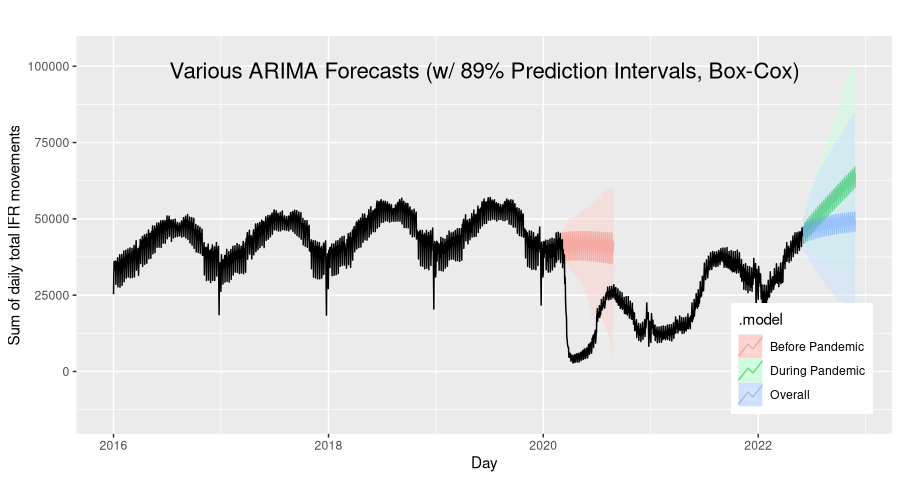
\includegraphics[width=.9\linewidth]{./media/arima.png}
\end{center}

As expected, the \texttt{during} model has a high trend, due to the world bouncing back. Heuristically, \texttt{during} would not be a very suitable model as it overshoots the values before lockdowns. However, the future is uncertain, and even the prediction intervals on \texttt{overall} capture higher-than-before values.
\end{document}